\documentclass[crop=false]{standalone}
\usepackage{graphicx}
\graphicspath{{images/}}
\usepackage[utf8]{inputenc}
\usepackage{blindtext}

\begin{document}



\section{Aplicaciones de Machine Learning en la Red Eléctrica Inteligente}
Este capítulo proporciona una visión general de las aplicaciones del aprendizaje automático en el sistema eléctrico, particularmente en la red eléctrica inteligente (SG por sus siglas en inglés). Dado que el crecimiento diario del sector eléctrico en el uso de energía está aumentando, es crucial que se produzca más energía sin dañar el medio ambiente y que se utilice de manera eficiente con las menores pérdidas posibles. Con la última tecnología, como la inteligencia artificial (IA) y el aprendizaje automático (ML por sus siglas en inglés), esto es alcanzable. Al combinar una infraestructura de medición de vanguardia, tecnologías de control y comunicación, la red eléctrica inteligente permite la recolección de enormes volúmenes de diversos tipos de datos relacionados con las operaciones de la red eléctrica. Los usos de los enfoques de ML en la red eléctrica inteligente se están volviendo más claros como resultado de las numerosas limitaciones de las tecnologías convencionales de modelado y optimización en el procesamiento y análisis de datos. La previsión de carga a corto y largo plazo, la evaluación de la estabilidad de la red eléctrica, la predicción de la fiabilidad y los problemas de seguridad en la red eléctrica inteligente y los sistemas eléctricos en general, son algunas de las áreas típicas donde se pueden aplicar los enfoques de IA y ML.
\section{ Introducción}
El rápido desarrollo y uso generalizado de tecnologías de información y comunicación más sofisticadas no sólo requiere nuevas prácticas energéticas, patrones de trabajo actualizados y formas de actividad económica, sino que también está transformando la demanda de electricidad. Se ha vuelto un desafío para las redes controlar la demanda de energía para usos domésticos e industriales debido al aumento de la población mundial y la expansión de las industrias. A medida que más empresas, hogares y sistemas energéticos dependen de soluciones alimentadas por electricidad, estas tecnologías ofrecen nuevas posibilidades para una gestión inteligente y flexible de la oferta y la demanda, pero al mismo tiempo plantean nuevas amenazas y preocupaciones. Problemas como cortocircuitos y fallos en transformadores pueden ser causados por la mayor demanda de energía en ciertos momentos del día. Es necesario estimar el consumo del cliente de patrones de uso para suministrar con éxito la energía y superar estos problemas con la transmisión de electricidad a través de redes convencionales. Una SG (Red Eléctrica Inteligente) puede transportar energía según la demanda anticipada utilizando inteligencia para estimar el consumo eléctrico. Una SG puede manejar varios problemas de la red convencional mediante la detección inteligente y la predicción, incluyendo la previsión de la demanda, reducir el consumo de energía y disminuir el riesgo de fallos por cortocircuitos, evitando pérdidas de vidas y propiedades.
El verdadero potencial de las SG ha sido desbloqueado por avances tecnológicos como el Internet de las Cosas (IoT), análisis de grandes datos, aprendizaje automático (ML) y redes inalámbricas de quinta generación (5G) y más allá. Como se muestra en la Figura 12.1, la SG tiene varios interesados y puede conectarse con varios otros sectores inteligentes, incluyendo ciudades, edificios, automóviles y plantas eléctricas inteligentes. Esta infraestructura de red modernizada, habilitada por el Internet de las Cosas (IoT), está construida alrededor de la conectividad. Sin embargo, la conectividad y comunicación constantes generan grandes volúmenes de datos que requieren metodologías significativamente mejores que las tradicionales. Aunque un sistema SG con integración de IoT puede ofrecer una transmisión de energía eficaz, costos de gestión reducidos, seguridad mejorada e integración de fuentes de energía renovable, lograr estas ventajas requiere análisis de grandes datos y enfoques de aprendizaje automático. La naturaleza conectada de la red inteligente resulta en la generación constante de datos que deben ser recopilados, almacenados y gestionados. Cada año, una típica empresa de distribución procesa miles de terabytes (TB) de datos nuevos. Los medidores inteligentes, equipos de medición de campo, unidades terminales remotas, enchufes inteligentes y termostatos programables son algunas de las fuentes de estos datos. Por lo tanto, el uso eficiente del análisis de grandes datos es esencial para crear modelos de negocio adecuados para los principales interesados y para la operación eficaz de las redes eléctricas del futuro.
Los ordenadores son entrenados para tomar decisiones basadas en experiencias utilizando un proceso de análisis de datos llamado aprendizaje automático. El aprendizaje automático ha surgido como una herramienta crítica para resolver problemas a medida que han aumentado los volúmenes de grandes datos. Numerosos enfoques de aprendizaje automático pueden ahora ser aplicados en aplicaciones de red inteligente gracias al continuo avance de las técnicas informáticas, particularmente en la gestión y análisis de datos. Complementa el sistema de red inteligente, que se basa en la adquisición, análisis y toma de decisiones basadas en datos, como el último componente. La red eléctrica inteligente puede funcionar como se espera porque las técnicas de aprendizaje automático ofrecen un enfoque efectivo para evaluar los datos y luego tomar las decisiones operativas correctas. La programación óptima futura, la generación de energía, la detección de fallos y la detección de intrusiones en la red son algunas de las características del aprendizaje automático.
Dado que la tecnología de red inteligente es tan sofisticada, hay muchas formas en que los atacantes pueden interferir con el sistema. Por lo tanto, se necesita una estrategia defensiva completa para abordar todas las amenazas y debilidades potenciales a las que una red inteligente pueda enfrentarse. Se ha demostrado que las técnicas de aprendizaje automático son una herramienta especialmente efectiva para prevenir ataques de denegación de servicio. La ciberseguridad se está convirtiendo en una preocupación seria en el sistema conectado de SG, con los dispositivos de IoT y los datos que contienen emergiendo como objetivos principales para los ataques. La fiabilidad y resistencia de los sistemas de red inteligente pueden ser mejoradas y potenciadas por el uso de métodos de IA y ML.

\begin{center}
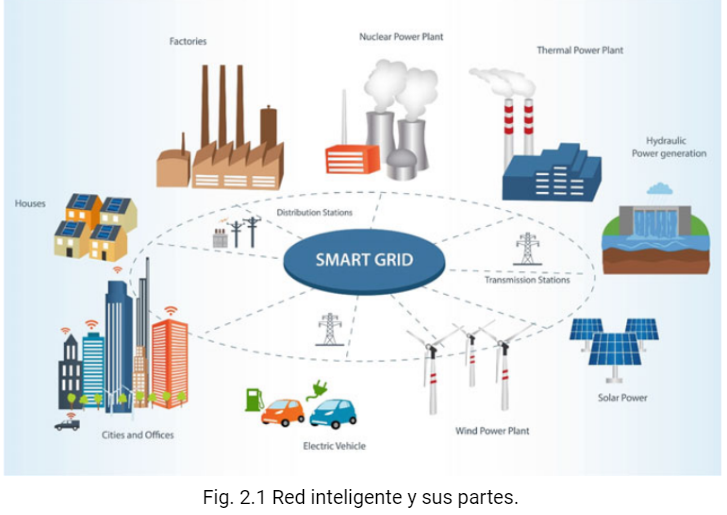
\includegraphics[width=0.9\textwidth]{images/foto_texto_traducido.PNG}

\end{center}

El aprendizaje automático tiene la capacidad de reconocer ataques, tomar medidas preventivas para solucionar problemas existentes y alertar a los profesionales de seguridad. Las técnicas de aprendizaje automático deben ser continuamente mejoradas para que la industria eléctrica avance hacia redes inteligentes, ya que su uso puede integrar sin problemas todos los componentes empleados. Así, se aseguran calidad, eficiencia y continuidad en sistemas eléctricos inteligentes además de fiabilidad.
Numerosas causas están presionando a las empresas de servicios públicos, y la infraestructura eléctrica está constantemente bajo estrés: la electrificación aumenta la demanda, especialmente por la expansión exponencial de los automóviles eléctricos; la energía renovable y la generación solar residencial están cambiando el lado de la oferta introduciendo nuevos tipos de fuentes de energía y cambiando la dirección del flujo de energía a través de las redes; las pérdidas y el tiempo de inactividad deben reducirse mientras que la eficiencia de la red debe aumentarse. Las empresas de servicios públicos están invirtiendo en tecnologías de red inteligente que proporcionan una mejor monitorización y gestión de la red con el fin de equilibrar la nueva oferta y demanda, más dinámicas.
El clima, la generación de energía renovable y el consumo de energía se predicen utilizando el aprendizaje automático. La variabilidad de fuentes de energía renovable como el sol y el viento es a menudo asombrosa. El sistema eléctrico y la gestión de la red están seriamente en peligro como resultado de esto. Pueden ocurrir desgloses del sistema si el suministro y la demanda de la red eléctrica no están perfectamente sincronizados.
Tanto los proveedores de servicios públicos como los clientes pagan un alto precio por esto. La oferta y la demanda pueden coincidir perfectamente cuando es posible predecir cuánta energía eólica y solar estará disponible en un momento particular. Los algoritmos de aprendizaje automático se entrenan en conjuntos de datos históricos, así como en datos recopilados de paneles eólicos o solares, para predecir con precisión el clima y las fluctuaciones de energía.
No podemos prevenir totalmente los grandes cortes debido a la complejidad e interconexión de las redes eléctricas actuales, pero debemos planificar y estar preparados para ellos más que nunca debido a nuestra dependencia de la energía.

\section{Técnicas de Aprendizaje Automático en Redes Inteligentes}

Se utilizan grandes volúmenes de datos en los enfoques de IA para construir máquinas inteligentes que son capaces de realizar operaciones que requieren inteligencia humana. A veces, se utiliza el aprendizaje automático (ML por sus siglas en inglés) de manera intercambiable con la inteligencia artificial (IA). Pero el ML es solo un método para desarrollar sistemas de IA (Fig. 12.2). Las redes neuronales, los sistemas expertos, la lógica difusa y el procesamiento de lenguaje natural son enfoques más generales para crear sistemas de IA.
En general, los enfoques de IA permiten una toma de decisiones rápida y precisa. En las aplicaciones de redes inteligentes, la inteligencia artificial (IA) es el proceso a través del cual las computadoras imitan los procesos cognitivos de los operadores de la red para proporcionar habilidades de auto-reparación. Pero en otras circunstancias, la IA podría no ser capaz de asumir el papel de los operadores de la red. Aunque el uso de la IA para mejorar los sistemas de redes inteligentes puede hacerlos más precisos, confiables y completos, todavía hay numerosos obstáculos por superar.
La división más general de ML se da en aprendizaje supervisado y no supervisado. El aprendizaje supervisado es un paradigma donde se ha examinado la relación entre entradas y salidas para predecir los resultados de nuevas entradas. El aprendizaje no supervisado es un tipo de aprendizaje automático en el cual se capturan las similitudes y diferencias entre conjuntos de datos no etiquetados. Dependiendo del tipo de variable que se está prediciendo, el aprendizaje supervisado puede dividirse: tenemos un problema de regresión en nuestras manos si el valor predicho es continuo. Por otro lado, se utiliza la clasificación cuando la variable a predecir pertenece a una de varias categorías separadas conocidas como clases. Estas clases pueden ser valores distintos con contenido cualitativo o cuantitativo.

\begin{center}
\includegraphics[width=0.9\textwidth]{images/foto_texto_traducido_2.PNG}

\end{center}

\begin{center}
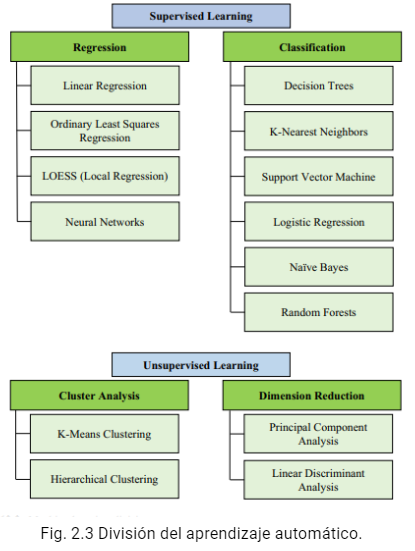
\includegraphics[width=0.8\textwidth]
{images/foto_texto_traducido_3.PNG}

\end{center}

Machine learning (ML) es una frase que describe cómo una máquina aprende a partir de los datos a los que tiene acceso y realiza predicciones. Está compuesto por múltiples algoritmos que utilizan un conjunto de instrucciones para evaluar los datos disponibles con el fin de generar predicciones y/o juicios que estén informados por los datos. Se diseñan y programan rigurosamente algoritmos específicos con un rendimiento previsto para el aprendizaje automático. Las predicciones sobre el consumo, la fijación de precios, la generación de energía, los horarios óptimos futuros, la detección de fallos, el control adaptativo, el dimensionamiento y la detección de intrusos de red durante una violación de datos son solo algunas de las características disponibles a través del aprendizaje automático.
Cuando se evaluó en el sistema de 39 buses de Nueva Inglaterra, Xu et al. propusieron una metodología de evaluación para medir la velocidad de cálculo. Con el objetivo de utilizar la enorme cantidad de datos producido por PMU, Wang et al. desarrollaron un nuevo algoritmo de máquina vectorial central (CVM, por sus siglas en inglés). Su sistema también fue probado en el sistema de buses de Nueva Inglaterra.
Los datos de la unidad de medición de fasores (PMU) y la micro unidad de medición de fasores (µPMU) para sistemas de transmisión pueden ser evaluados usando aprendizaje automático con propósitos como detección de frecuencia y visualización del sistema. Junto con otros programas como la herramienta de evaluación de riesgo de vuelo libre y la herramienta de validación del modelo de planta de energía (PPMV), el aprendizaje automático puede ser utilizado para estos objetivos. Una amplia variedad de técnicas de aprendizaje automático se están implementando en varias etapas de las redes inteligentes basadas en sistemas de energía renovable, abriendo un campo de estudio completamente nuevo.
Las máquinas de vectores de soporte (SVM, por sus siglas en inglés), por ejemplo, han sido ampliamente utilizadas para resolver varios problemas relacionados con sistemas de energía renovable y han dado lugar a varias optimizaciones y estrategias de predicción en redes inteligentes.
Recientemente, desarrollaron un método rápido y preciso para monitorear eventos de calidad de energía (PQ) en una red inteligente basada en aprendizaje automático. Para determinar patrones y preferencias de uso en una red inteligente, Li et al. emplearon aprendizaje automático para examinar las preferencias del usuario.
Remani et al. mostraron cómo programar cargas residenciales teniendo en cuenta las fuentes de energía renovable y todos los posibles tipos de tarifas. El uso del aprendizaje automático y el diseño wavelet para la identificación de islanding en sistemas generadores distribuidos fue investigado. La aplicación de optimización por enjambre de partículas (PSO, por sus siglas en inglés) se sugiere  para mejorar la estabilidad para el islanding no planificado en microgrid. Esta etapa de estabilización ocurre antes del análisis de grandes datos para rastrear e identificar tales episodios de islanding. Jurado et al. sugirieron un sistema híbrido de gestión de la demanda en que hace uso de selección de características basada en entropía, aprendizaje automático y computación blanda.
Se examinó cómo entrenar redes de funciones de base radial comunes para la predicción de carga usando una variedad de técnicas, incluyendo la máquina de aprendizaje extremo, regresión vectorial de soporte, función neural de base radial de segundo orden mejorada y corrección de errores.
En comparación con sistemas actuales como redes neuronales superficiales (SNN) y doble estacional Holt-Winters (DSHW), Ryu et al. sugirieron una técnica de pronóstico de carga de red neuronal profunda (DNN) para predicción a corto plazo en el lado de la carga que reveló hasta un 29 por ciento de error reducido.

\subsection{Pronóstico de Carga}

La programación y gestión de la red inteligente se están volviendo más complejas debido a la creciente integración de fuentes de energía renovable, incluidas la solar, eólica y la energía de las mareas. Para la planificación y operación en sistemas eléctricos contemporáneos, el pronóstico de carga es esencial como uno de los elementos fundamentales para mantener la estabilidad e inteligencia del sistema eléctrico. Si la carga es no estacionaria, el pronóstico preciso, que es beneficioso para reducir los costos de producción y conservar la electricidad [40], es muy difícil.
Se pueden distinguir tres grados de pronóstico de carga (LF) según el tiempo que se debe proyectar: pronóstico de corto plazo (STLF) que pronostica la carga de minutos a horas; pronóstico a medio plazo (MTLF) que pronostica la carga de horas a semanas; y pronóstico a largo plazo (LTLF) que pronostica la carga para años. Además, características adicionales como el clima, la hora, la estación, los eventos, el tipo de cliente y el calendario académico pueden afectar al LF. Por lo general, los pronósticos MTLF y LTLF se modelan como funciones de datos históricos sobre el consumo de energía además de otras variables como el clima, la clientela y la información demográfica [42]. La planificación de futuras centrales eléctricas y la representación de la dinámica del sistema eléctrico pueden hacerse usando MTLF y LTLF. Se desarrollan y utilizan numerosas estrategias para el LF del sistema eléctrico basadas en los datos proporcionados por los medidores inteligentes.
Qiu et al. proponen una estrategia híbrida de aprendizaje incremental que combina la transformación wavelet discreta, la descomposición de modo empírico y la red funcional de vectores aleatorios.
Li et al.  ofrecen un modelo que utiliza una técnica de conjunto para combinar tres enfoques base de STLF, y las pruebas demuestran la eficacia del modelo para STLF. Sin embargo, es necesaria una mayor verificación para la selección de técnicas básicas del enfoque de conjunto.
Hay varias técnicas basadas en DL para abordar los problemas de LF. Recientemente se han empleado DNNs para recopilar información prospectiva para modelos predictivos. Sin embargo, el método ANN a menudo se encuentra con problemas de sobreajuste y mínimos locales. Shi et al. presentaron un RNN profundo basado en pooling para STLF para combatir el sobreajuste.
Moon et al. utilizaron un método de conjunto que combina varios modelos DNN con diferentes números de capas ocultas para lograr un rendimiento general mejor eliminando los modelos con bajo rendimiento.
Debido a la inclusión de muchas CNNs, la sobrecarga computacional es una limitación. He, Deng y Li sugieren una DBN integrada con modelos Copula paramétricos para estimar la demanda horaria de un sistema eléctrico en una región urbana de Texas. Los resultados muestran la eficacia del método en comparación con las redes neuronales, SVR y ELM. Hafeez et al. Presentan un enfoque híbrido utilizando la optimización GWDO y FCRBM como módulo de entrenamiento. El modelo se muestra preciso superando al algoritmo de vanguardia. Aly desarrolló una técnica híbrida de clustering basada en redes neuronales wavelet (WNN) y esquemas ANN, que demostró un rendimiento superior al compararlo con los métodos de clustering existentes.
Para prever la demanda de energía, planificar el sistema y programar el crecimiento de las unidades generadoras en los sistemas eléctricos, se utiliza LTLF. A menudo dura desde unos pocos años hasta varias décadas.
Al prever la relación entre la demanda de carga y diversos factores ambientales, Nalcaci et al. demuestran que la técnica MARS proporciona resultados más precisos y fiables que los modelos ANN y LR. Para LTLF, Ali et al. utilizaron un nuevo modelo híbrido fuzzy-neuro. Dong et al. presentan una técnica híbrida basada en LSTM y la unidad recurrente controlada (GRU) con alto rendimiento para LTLF para abordar los problemas de gradientes desaparecidos y explosivos de LSTM. En Kumar et al., se implementó un modelo híbrido compuesto por LSTM y GRU utilizando Apache Sparks con el propósito de ajustar hiperparámetros. Bouktif et al. También sugieren un modelo LSTM-RNN para este propósito. Seis métodos de aprendizaje automático (ML) frecuentemente utilizados fueron examinados por Sangrody et al.: ANN, SVM, RNN, KNN, GPR y la red neuronal de regresión generalizada (GRNN). Para LTLF, ANN tuvo un mejor rendimiento que los otros cinco enfoques.

\section{Red Inteligente y Sociedad 5.0}

En años recientes, hemos presenciado cambios significativos en los marcos económicos y sociales, así como en las estructuras industriales debido a la integración generalizada de fuentes de energía renovable, desarrollo de tecnologías de información y comunicación (TIC), globalización, cambios en los valores de las personas y otros factores. Con el objetivo de construir nuevos valores que aborden estos cambios económicos y sociales, ofrecer una visión futura para una sociedad súper inteligente que resultaría en una existencia digna y abordar problemas sociales antes que el resto del mundo, el gobierno japonés ha presentado su iniciativa "Sociedad 5.0".
En la Sociedad 5.0, las personas estarán en el centro de la vida diaria, y cada pequeña comunidad establecerá su propio sistema energético. Se trata de construir un mundo en el cual la imaginación de las personas en todos lugares sea utilizada para resolver diversas preocupaciones energéticas y generar nuevo valor, alejándose del modelo centralizado uniforme basado en la expansión de escala que ha sido empleado hasta este momento.
También es necesario integrar y coordinar numerosas infraestructuras, construir sistemas energéticos adecuados para la población local y realizar cambios radicales en las estructuras económicas, sociales e industriales. Sin embargo, debido a la distribución regional desigual y los cambios temporales provocados por la integración de la energía renovable, será un desafío sofocar el intercambio de suministro-demanda de energía y valor en una sola comunidad local. Como resultado, se requerirá que el sistema de energía a granel conecte diversas comunidades locales y gestione el sistema en general.
Las redes de energía y de energía a granel de las comunidades locales dejarán de funcionar con normalidad en estas circunstancias, lo que requerirá su reconstrucción basada en la coexistencia. Se deben preparar una amplia gama de opciones tecnológicas para lograr este objetivo. El sistema eléctrico se verá significativamente impactado, en particular, por las variaciones de producción de energía solar y eólica, etc. Por ejemplo, es necesario desarrollar nuevas tecnologías de control como inversores inteligentes para energías renovables y plantas de energía virtual (VPPs).
Al permitir que el control de energía de las comunidades locales ejecute una parte de la función de coordinación de oferta y demanda, actualmente gestionada por instalaciones de energía térmica y de almacenamiento bombeado, se puede aprovechar al máximo el potencial de los sistemas existentes para optimizar la rentabilidad del sistema social.
Para ello, es esencial desarrollar infraestructuras IT que conecten las grandes instalaciones de las comunidades locales, planes de control para maximizar sus impactos, incentivos y otras regulaciones.
En la Sociedad 5.0, la IA almacena información obtenida del espacio físico en el ciberespacio, permitiendo el análisis de datos en el futuro con el uso de HCPSs. La última generación de IA, conocida como HCPSs, se basa en ontología y tiene en cuenta todas las interacciones humano-máquina. Además, esta técnica proporciona nueva información a los negocios y a la sociedad al considerar elementos ambientales y biológicos de las personas, que antes eran inaccesibles. Para que la Sociedad 5.0 logre un equilibrio entre el progreso económico y la solución de problemas sociales, la ciencia debe imitar las estructuras y procesos observables en la evolución biológica.
La Industria 4.0 se centra en el uso de diversas tecnologías digitales y basadas en la web para recopilar y analizar datos, mientras que la Industria 5.0 se centra en el cambio geoestratégico provocado por la biología sintética.
Con el objetivo de establecer procedimientos sin fallos para la integración de la IA en las ciudades inteligentes, el concepto es crear ciudades dinámicas que estén estructuradas en función de las circunstancias ambientales y que utilicen productos, energía y servicios basados en la biología. El objetivo es alinear completamente los procesos de producción con los requisitos medioambientales y las demandas de los clientes, así como mejorar continuamente los datos del proceso, los servicios y los productos, así como las infraestructuras conectadas, los sistemas inteligentes y los sistemas de registro. Además, utilizando el conocimiento de la Sociedad 4.0 y los parámetros confirmados en el área física relevante, la programación de datos descrita aquí permite la creación de redes neuronales artificiales para la toma de decisiones.
Un marco teórico para el desarrollo urbano, las ciudades inteligentes se basan en la explotación del capital humano, social y tecnológico. El concepto de una sociedad inteligente puede expandirse más allá de las ciudades inteligentes; de hecho, la Sociedad 5.0 puede evaluar las necesidades humanas utilizando procedimientos estandarizados en conjunción con la IA. Como resultado, una sociedad basada en el conocimiento y habilitada digitalmente debe esforzarse por lograr la sostenibilidad social, ambiental y económica.
La creación de ciudades inteligentes y una sociedad inteligente depende del crecimiento del capital humano y social, lo que requiere enfoques novedosos para procesos que sean predictivos y adaptables. El objetivo es diseñar una economía basada en el conocimiento con una infraestructura digital que pueda cooperar y permitir interacciones dinámicas en tiempo real entre múltiples subsistemas de ciudades inteligentes.
Actualmente, hay decenas de explicaciones de lo que es una ciudad inteligente o inteligente en la literatura, pero no hay un consenso general. En cualquier caso, se puede decir que las ciudades inteligentes son sociedades centradas en el ser humano donde la IA elige procesos para lograr las mejores condiciones de calidad de vida mediante el uso de fábricas inteligentes equipadas con dispositivos inteligentes (sensores/actuadores), controladores lógicos programables (PLC), sistemas de gestión de procesos y ejecución de fabricación, planificación de recursos empresariales SW y HCPS.
El concepto es que los pedidos pueden realizarse desde cualquier lugar de la red y la tecnología plug-and-produce, basada en infraestructuras inteligentes y ontologías, puede gestionar y reorganizar los procesos de producción de forma remota. Como resultado, el equipo industrial puede integrarse, cambiarse o reemplazarse sin necesidad de ayuda de recursos humanos expertos para la reconfiguración del sistema. De hecho, la tecnología plug-and-produce permite la colaboración inteligente con otros dispositivos al permitir la reconfiguración e interacción inteligente de dispositivos inteligentes conectados con el PLC.

\section{Conclusión}

A medida que el sistema tradicional de la red eléctrica evoluciona hacia un sistema de red inteligente, los procedimientos convencionales del sistema de energía enfrentan desafíos al procesar y evaluar los enormes volúmenes de datos. Como resultado, se están logrando resultados prometedores a través del desarrollo e implementación de enfoques de IA y ML.
Dado el ritmo de desarrollo de la tecnología de IA, se anticipa que las aplicaciones de red inteligente de IA y ML enfrentarán algunas de las siguientes dificultades principales: una recolección insuficiente de muestras de datos, la confiabilidad aún debe mejorarse, se deben cumplir los requisitos de infraestructura y falta de algoritmos adaptados a ciertas industrias.
En conclusión, en comparación con la red tradicional, la confiabilidad y resistencia de los sistemas de red inteligente están siendo mejoradas mediante el uso de aplicaciones de estos nuevos enfoques. Aunque se han propuesto diversas soluciones basadas en datos para abordar los problemas con las redes inteligentes, todavía existen muchos obstáculos significativos, como la inclusión de fuentes de energía renovable, mantener la privacidad y seguridad de los datos, el almacenamiento y análisis rápido de datos masivos, limitaciones de algoritmos de IA, etc.
Sin embargo, las nuevas tecnologías seguirán desafiando a las redes de energía convencionales en los años venideros. Es fácil ver cómo las soluciones de red inteligente pueden beneficiar no solo a los proveedores y clientes de energía, sino también a nuestras comunidades y al medio ambiente con características como conectividad sin interrupciones, control remoto, optimización del rendimiento, mantenimiento de reducción de costos y reducción de residuos. Las soluciones de red inteligente son el presente de la energía porque son escalables, seguras y económicas.


\end{document}

